\chapter{Logic}
%\begin{flushright}
%\end{flushright}
\minitoc

Note:  This chapter is currently very chaotic because of a re-organization effort.  $\mathcal{Z}$ is no longer considered a foundational part of the logic.

\section{Background}

\subsection{Turing completeness}

\textbf{Undecidability of FOL.}

\subsection{$\lambda$ calculus}

(See Wikipedia: \href{http://en.wikipedia.org/wiki/Lambda_calculus}{Lambda calculus}).

\textbf{Bound variables:}  In the abstraction $(\lambda x.t)$ we call $x$ the bound variable and $t$ the body.  Every occurrence of $x$ in $t$ is \textbf{bound} by the abstraction.  Conversely, an occurrence of a variable $y$ is \textbf{free} if it is not bound, eg in $(\lambda z.(\lambda x.(yx)))$.

\textbf{Head-normal form:}  A $\lambda$ term is in head-normal form if, for $m \geq 0$ and $n \geq 0$, it can be expressed as:
$$\lambda x_1 ... x_m . x t_1 ... t_n$$.
The variable $x$ may either be free or bound (one of $x_1,...,x_m$).

\textbf{De Bruijn indexes.}

\textbf{Director strings.}

\subsection{Combinatory logic}

(See Wikipedia: \href{http://en.wikipedia.org/wiki/Combinatory_logic}{Combinatory logic}).

Bound variables -- why they are confusing?

\subsection{Term-rewriting systems}

\subsection{Simple type theory}

\subsection{Higher-order logic}

\textbf{Standard semantics and general semantics (of higher-order logic).}

Why Henkin semantics is a reduction to FOL?

\subsection{Model theory}

\subsection{Proof theory}

\subsection{Deduction systems}

\textbf{Hilbert systems.}

\textbf{Natural deduction.}

\textbf{Sequent calculus.}

\textbf{Tableau.}

\textbf{Resolution.}

\subsection{Paradoxes in logic}

\textbf{Liar's paradox.}

\textbf{Skolem's paradox.}

\textbf{Tarski's paradox.}

\textbf{Non-axiomatizability.}  ``First order logic has an effective notion of proof which is complete w.r.t. the intended interpretation.  This is the content of Godel's completeness theorem.  As a result, the set of (Godel numbers of) universally valid first-order formulas is recursively enumerable.''  But ``the set of second order validities is not arithmetically definable let alone recursively enumerable and hence that an effective and complete axiomatization of second-order validity is impossible'' \citep*{Benthem}.

\subsection{Functional programming}

\section{Logic and pre-logic}

Designing the perfect logic is nearly impossible, as witnessed by the proliferation of alternative logics in recent decades.  \textbf{Pre-logics}, or logical frameworks, are attempts to reduce logics to simpler computational mechanisms, and thus to tackle the problem in a general way.

The candidates for pre-logics include:
\begin{compactenum}[\textbullet ]
\item $\lambda$ calculus
\item combinatory logic
\item term-rewriting systems
\item grammars
\item programs (such as genetic programs)
\item etc
\end{compactenum}

The basic configuration of a system with pre-logic is like this:
\begin{figure}[H]
\centering
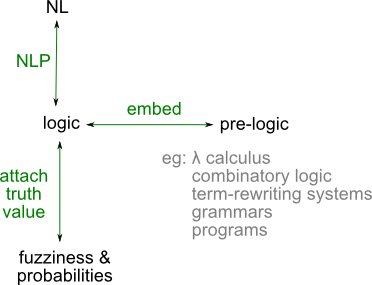
\includegraphics[scale=0.7]{prelogic.png}
% \caption{Prelogic}
\end{figure}
NL should be translated into logic because logic is closer to NL than pre-logic.  What really distinguishes ``logic'' from pre-logic is the notion of \textbf{propositions}, which is a unit of meaning to which we can attach \textbf{truth values}.  A proposition such as \formula{male(john)} is a ``complete'' entity of meaning, as opposed to the predicate \formula{male} which is incomplete, or ``syncategorematic''\footnote{The term syncategorematic has several meanings, here I mean any component of a sentence that is not a proposition.}.  This distinction is important because fuzziness and probabilities should be assigned to the logic rather than pre-logic.

The problem with the above configuration is, if the pre-logic is fixed and the logic is allowed to be dynamically learned, then it may be difficult to work with such a dynamically changing logic, in particular to assign fuzzy-probabilistic truth values to it, or to translate NL to it.

\section{Uncertainty}

Reasoning under uncertainty is a vast and nightmarishly complex topic in AI.  Simon Parsons's book \citep*{Parsons2001} contains a very good survey of uncertain reasoning, but even that is not exhaustive.  We may look at the following taxonomy of ``ignorance'' proposed by \citep*{Bosc1997}:
\begin{figure}[H]
\centering
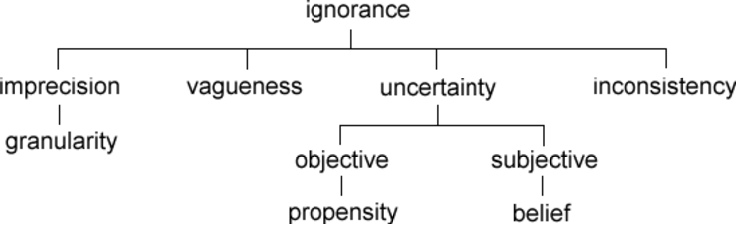
\includegraphics[scale=0.7]{IgnoranceTaxonomy.png}
\caption{taxonomy of ignorance}
\end{figure}

At first blush, classical logic appears to be sufficient for AGI.  Some AGI designers prefer to use crisp logic as the base and plan to build $\mathcal{P}$ and $\mathcal{Z}$ upon crisp logic.  But this may be a sign of not facing problems and not having sufficient understanding of fuzzy-probabilistic logics.  To represent $\mathcal{P}$ and $\mathcal{Z}$ logic \textit{in} crisp logic is like writing an entire $\mathcal{P}$-$\mathcal{Z}$ inference engine in Prolog, complicated by the fact that the crisp logic would be somewhat different from Prolog and so may be even harder to program in.  Also, the ``truths'' known by the AGI will then be different from the truths as represented in the crisp logic --- the former would be ``floating'' above the latter;  This creates unnecessary indirectness.  I will give other reasons in \S\ref{sec:whyZ} and \ref{sec:whyP}.

\textbf{Why not include other uncertainty measures besides $\mathcal{P}$ and $\mathcal{Z}$?}

There are other theories of uncertainty, such as possibility, belief functions, and rough sets.  The reason I chose $\mathcal{P}$ and $\mathcal{Z}$ is because they are simple and best understood.  There has been attempts to create systems where the user can create a flexible number of uncertainty measures, but one problem of such systems has been pointed out in \citep*{Parsons2001}:  If we have 3 uncertainty measures, say ``cloud'', ``mist'', and ``fog'', there would be a need to provide mixed inference rules for ``cloud-mist'', ``cloud-fog'' etc, a total of $n^2$ possibilities.  I have worked out the combination of $\mathcal{B}$, $\mathcal{P}$ and $\mathcal{Z}$ and found that it involved considerable efforts.

\section{Nonmonotonicity and defeasible reasoning}
\label{sec:exceptions}

One can create defeasible logics from classical logic, for example Reiter's \textbf{default logic} and McCarthy's \textbf{circumscription}.  But the classical approaches seem to require enumerating all possible exceptions, which is impractical.

\textbf{2 examples:}

\textbf{A.}\\
\textit{
1. John is usually very punctual.\\
2. Therefore, John will arrive at the airport on time.\\
3. John has an accident en route to the airport, and dies.\\
4. Therefore, John will NOT arrive on time.\\}
Will John arrive on time?

\textbf{B.}\\
\textit{
1. Mary has cybersex with many partners.\\
2. Cybersex is a kind of sex.\\
3. Therefore, Mary has many sex partners.\\
4. A person who has many sex partners has a high chance of STDs.\\
5. Therefore, Mary has a high chance of STDs.}

What's wrong with example B?  On the one hand, we should admit that cybersex is sex (it is a borderline case), but it lacks certain prominent features of sex, such as physical contact (which is not necessarily a \textit{defining} feature of sex).  Thus, if we carry on reasoning with the idea that cybersex is sex, we may get unsound conclusions.  The key to resolving this problem is to recognize ``cybersex is sex'' with \textbf{qualifications} such as ``it is sex without physical contact''.

If we have a rule that ``sex transmits certain diseases'', we may have to attach the exception ``only if the sex involves physical contact''.  In the end, our rules may be inundated with possibly infinitely many exceptions.  How can we get out of this problem?

\citep*{Wang1994}, \citep*{Wang2006} in NARS provided a solution.  His idea is not to store the exceptions to rules, but instead allow a \textit{multitude} of rules to fire, calculate the ``confidence'' (\S\ref{sec:confidence}) of each conclusion, and pick the conclusion with the highest confidence.  This allows us to handle exceptions relatively easily.

For the example:
\begin{eqnarray}
X \PimpL A \nonumber \\
X \PimpL B \nonumber
\end{eqnarray}
Pei Wang's idea is to calculate the combined conditional probability by weighing each individual conditional probability with their associated \textbf{confidences} (\S\ref{sec:confidence}):
$$ P(X|A,B) = \frac{ P(X|A)c_A + P(X|B)c_B }{ c_A + c_B } $$
which is a nice idea\footnote{Except that NARS truth values do not conform to probability theory.}, but Abram Demski came up with an alternative idea that is more in accord with Bayesianism.  The idea is to reconstruct $P(X|A,B)$ from the marginal conditionals $P(X|A)$ and $P(X|B)$ and priors $P(A)$ and $P(B)$.  This is achieved by applying Bayes' rule twice:
\begin{eqnarray}
P(X|A,B) &=& \frac{P(A,B|X)P(X)}{normalization} \nonumber \\
         &=& \frac{P(A|X)P(B|X)P(X)}{normalization} \nonumber \\
         &=& \frac{P(X|A)P(A)P(X|B)P(B)}{P(X) \; normalization}
\end{eqnarray}

\{ To-do:  Abram's solution seems problematic, I'm discussing it with him... \}

\section{Equality}
\index{equality}  \index{identity|see{equality}}
\label{sec:equality}

A problem with equality is illustrated by the classic example ``Morning Star / Evening Star''.  This is a similar example and its rendition in logic:\\
\tab
\begin{tabular}{l|l}
\textit{``Clark Kent is Superman.''}               & \formula{clark-kent = superman} \\
\textit{``Superman can fly.''}                     & \formula{can-fly(superman)} \\
\textit{``Mary does not know that Clark Kent is Superman.''} & $\neg$ \formula{know(mary, "clark-kent = superman")} \\
\textit{``Mary knows that Superman can fly.''}     & \formula{know(mary, can-fly(superman))} \\
\textit{``Mary does not know that Clark Kent can fly.''} & $\neg$ \formula{know(mary, "can-fly(clark-kent)")}
\end{tabular}

Perhaps the solution is that \formula{"clark-kent"} (in quotes, ie, the Clark Kent that Mary knows) is not equal to \formula{clark-kent} (without quotes, ie, the real Clark Kent).

\section{Modal logic}
\begin{flushright}
\emph{Modality, si! Modal logic, no!}\\
--- John McCarthy
\end{flushright}

My view is to use predicates to represent modality instead of using modal logics.  This view was first advocated by \citep*{McCarthy1997}.

One argument for the use of modal logic arises from the previous example:\\
\begin{tabular}{l|l}
\hspace*{1cm} \textit{``Mary believes Superman is dead.''} & \formula{believe(mary, dead(superman))}\\
\hspace*{1cm} \textit{``Superman is Clark Kent.''} & \formula{superman = clark-ken}\\
\hspace*{0.7cm} * \textit{``Mary believes Clark Kent is dead.''} & \formula{believe(mary, dead(clark-ken))}
\end{tabular}\\
but Mary may not know that Superman is Clark Kent.  This problem can be resolved as in the last section (\S\ref{sec:equality}).

\section{Shortcomings of the current logic}

1.  \textbf{Binary vs $\mathcal{P/Z}$.}  It may be desirable to have binary logic alongside $\mathcal{P/Z}$ logic.  $\mathcal{P/Z}$ reasoning is suitable for common-sense concepts, whereas binary reasoning is good for \textit{programmatic}
\footnote{Ie, binary logic makes programming easier}
or computational reasons.  However, one unsolved problem is that many common-sense concepts appear to be binary but are fuzzy upon close inspection (eg male/female, dead/alive).  The question is how to let binary and fuzzy concepts coexist in the same logic.

2.  \textbf{First-order vs Higher-order logic.}  Let us admit outright that FOL as a KR scheme is insufficient for common-sense reasoning and thus AGI.  But I also have the impression that second-order logic would be sufficient for most common-sense reasoning purposes.

With some tricks (such as reification, \S\ref{sec:reification}), FOL may be able to deal with second-order reasoning.

Another trick is that the FOL reasoner can ``escape'' to a meta-reasoner when higher-order constructs are needed.  This will be taken up on the chapter on meta-reasoning, \S\ref{ch:meta-reasoning}.

As a more satisfactory long-term solution, we are currently working on creating a $\mathcal{P(Z)C}$ HOL, see \S\ref{sec:HOL}.

%With P and Z, the AGI can express ideas such as:\\
%\hspace*{1cm} ``Mary is \underline{probably} \underline{fairly} tall.''

\section{$\mathcal{B}$: binary logic}
\label{sec:binary-logic}

My intuition is that common-sense reasoning involves mainly $\mathcal{B}$, followed by $\mathcal{Z}$, and $\mathcal{P}$ is relatively rare.

%Horn clauses:  P and Z rules can be expressed in Horn form only.  But it seems that we can use general resolution for B rules, no?  Or, perhaps I want to use something similar to Horn resolution for P and Z?

%Each rule will enable one inference step, so the logic is almost truth-functional.  The problem is the intermediate results... I only know how to do that in B form.  Maybe we can keep a set of disjunctions of truth values?

%In B logic the proof procedure keeps a current clause / or a line of clauses.  In Bayes net we have a query variable and the algorithm finds its P value.  Z logic may be similar to B logic because it's truth functional?

%Perhaps we can work out the general case of a query variable of any TV type?  If we draw a B rule that's easy.  If Z rule, then we have a few Z variables as goals.  They need Z rules to fulfill, but what if we have a B rule for one of the sub-goals?  Then we need to translate the B value to Z value.  We can only do that via P(Z).  So we have a P(Z) value as one of the subgoals.  This may cause the head of the rule to become P(Z) too.  It seems there is a tendency for all TVs to become P(Z).
%That will actually back-propagate along the proof sequence.

%Things may be even worse for a P rule.  The application of the rule requires other numbers.  

\section{Meta-reasoning}
\begin{flushright}
\emph{I think I think, therefore I think I am.}
\end{flushright}

The term ``meta-reasoning'' may refer to 2 things:\\
1. The ability to \textbf{reason about reasoning}, which is what this chapter is concerned with;\\
2. Scheduling reasoning tasks to achieve best results with limited computational resources (I have not thought about this problem yet).

An excellent survey of meta-reasoning in the \#1 sense is \citep*{Constantini2002}.

In the Tell-Learn loop, we see that we need a special predicate credible() to increase the probability of a statement via a side-effect.  But that may not be the only meta-reasoning move we can make.

Another example is the $B \leftrightarrow Z$ conversion of ``traitor'' and ``patriot'' (\S\ref{sec:PZ-meta-reasoning}).

\section{Higher order logic}
\label{sec:HOL}

The HOL formulation that I am most familiar with is \citep*{Lloyd2003}.  It uses \textbf{typed lambda calculus} to represent logical formulae.  This representation is specifically developed for use as a logic programming language (Escher) and for inductive learning.

Interestingly, Lloyd uses a form of algebraic logic that is similar to what I do with $\mathcal{P(Z)C}$ logic, ie, its statements are of the form $H = B$ where $H$ is the head and $B$ is the body.  In essence this is the Prolog / Horn tradition.

\{ TO-DO:  formulate a $\mathcal{P(Z)C}$ HOL \}

\label{sec:PZ-meta-reasoning}

One example of meta-reasoning pertinent to fuzziness is:\\
\hspace*{1cm} S1: ``You are either a patriot or a traitor.''\\
\hspace*{1cm} S2: ``No, I can be slightly patriotic or slightly traitorous.''

In S1 the predicates \textit{patriot} and \textit{traitor} have binary character.  In S2 they have fuzzy character.

\underconst
